% This is samplepaper.tex, a sample chapter demonstrating the
% LLNCS macro package for Springer Computer Science proceedings;
% Version 2.20 of 2017/10/04
%
\documentclass[runningheads]{llncs}
%
\usepackage{graphicx}
\begin{document}
%

\title{Smart Library}

\author{Group 25: Bhagyalaxmi \and
Divya \and
Jerome}

\institute{Service Computing Department, IAAS, University of Stuttgart
\newline\email{st164379@stud.uni-stuttgart.de}
\newline\email{st164388@stud.uni-stuttgart.de}
\newline\email{st1164430@stud.uni-stuttgart.de}}
%
\maketitle              % typeset the header of the contribution
%
%
%
%
\section{Introduction}
Expeditious urbanization is leading to smarter cities with the intention to provide core infrastructure and a decent quality of life to its citizens, a clean and sustainable environment. Smartness can be established in any sector of the urban area: be it in an office, school, transportation infrastructure, library etc. 
Our idea is centralized to a library with focus on energy consumption, security, safety and comfort of its occupants. The sensors provide the current information about the temperature, humidity, light, motion in the library. The raw data  is transformed into context data by the input drivers. Energy consumption is controlled prudently by handling the lighting system, HVAC and burglar system dynamically after performing modification on the context data. Security is obtained by the alarming system in case of unexpected and malicious entry into the environment under consideration during closed hours.





\section{System architecture}
Fig.1 gives the System Architecture
\begin{figure}
\begin{center}
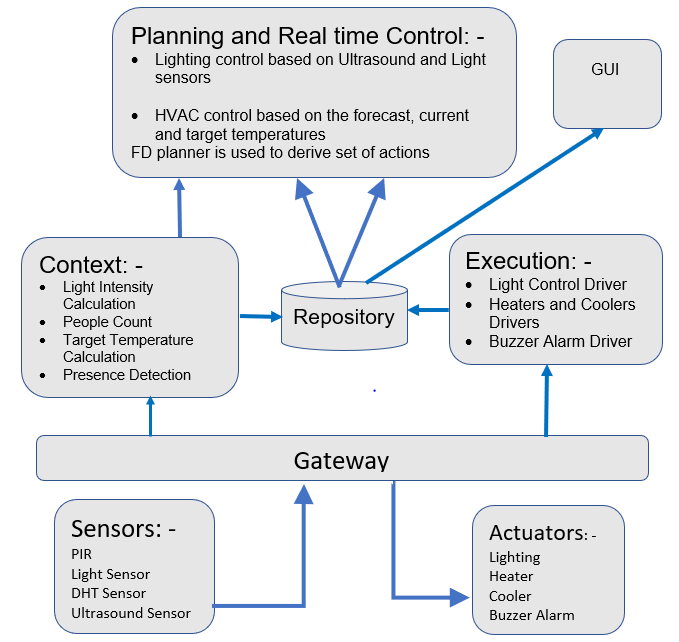
\includegraphics[scale=1]{fig1}
\caption{System Architecture}
\end{center}
\end{figure}
\section{Set-up and Implementation}

\textbf{SW and HW structure:}
Hardware Used: RaspberryPi Pi3 B+ with Groove Pi set and Plugwise Set.
Raspberry Pi is used as the central Gateway of the System which interacts with the sensors and actuators and also with the server for data storage. Figure 2 and 3 give the software and hardware designs respectively. A GUI is implemented in the server side for displaying the current system Status and also to plot the recorded data. 


\begin{figure}
\begin{center}
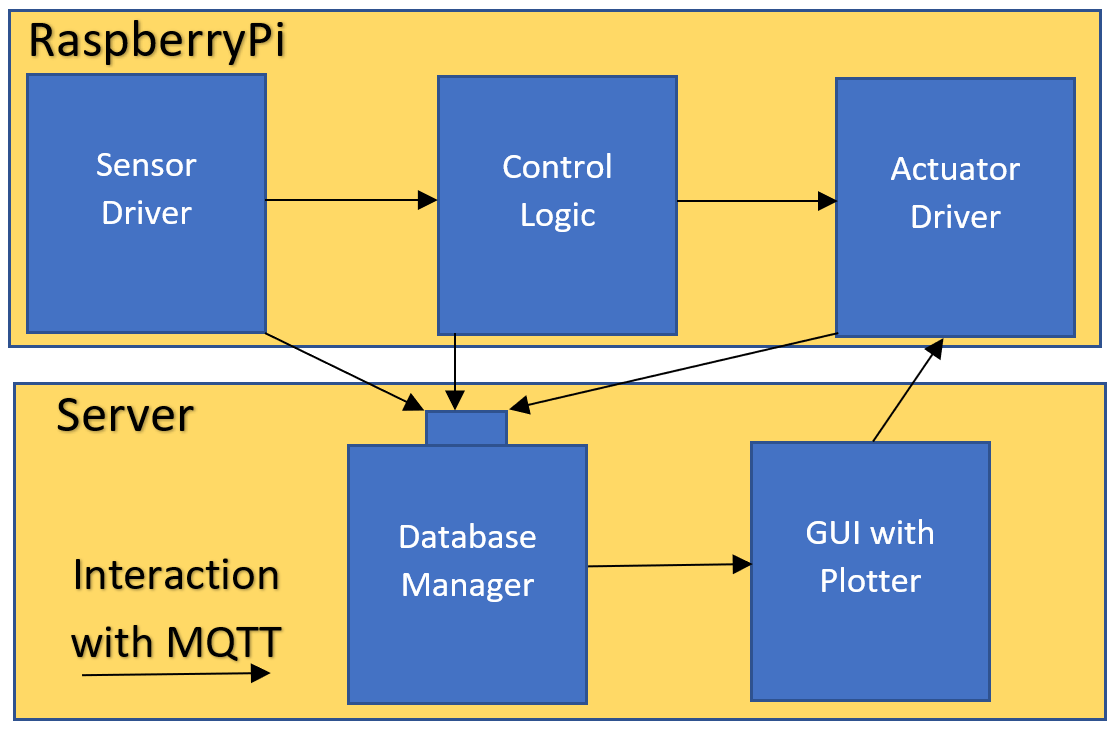
\includegraphics[scale=0.5]{fig3}
\caption{Software Design}
\end{center}
\end{figure}
\begin{figure}
\begin{center}
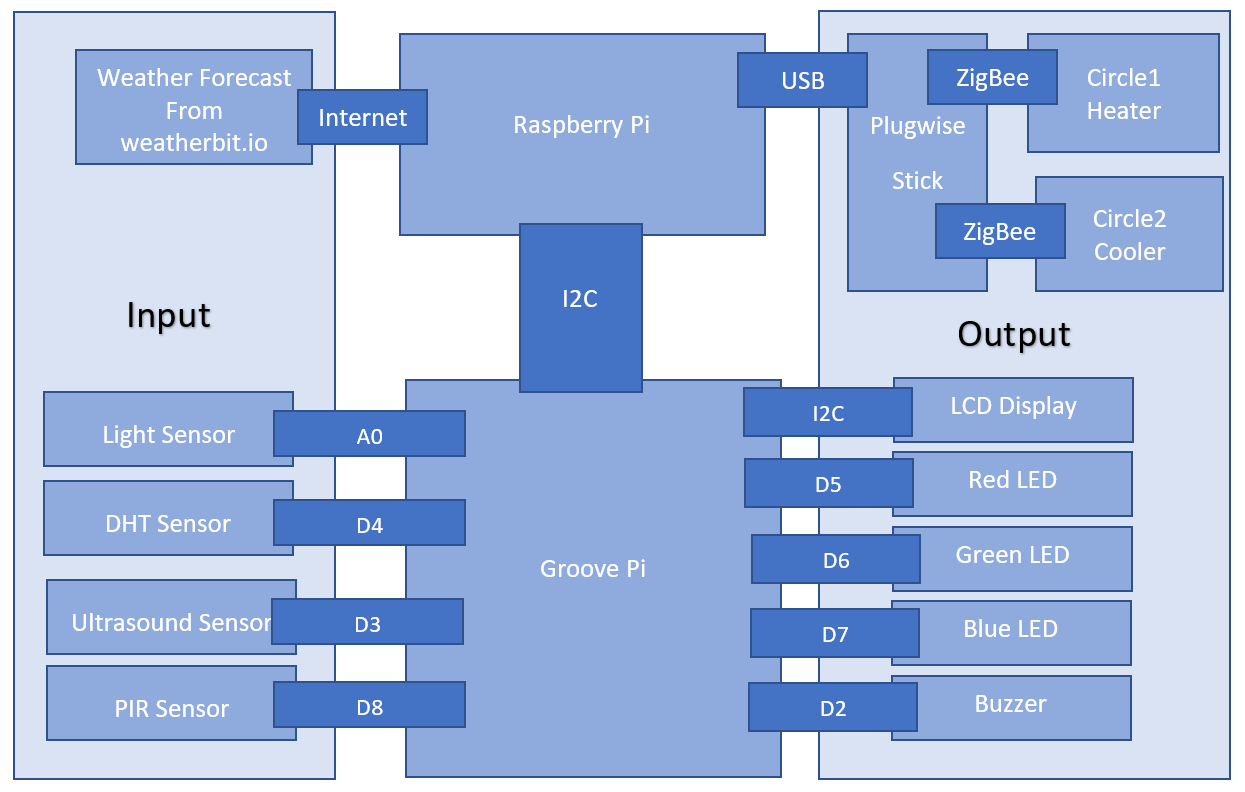
\includegraphics[scale=0.5]{fig4}
\caption{Hardware Design}
\end{center}
\end{figure}
\vspace{3mm}
\textbf{Working of our Smart Library}:
\vspace{5mm}
\newline\textbf{People Count}:
To efficiently control the lighting and heating of a building we should first be aware of the number of people inside the building. Here we use ultrasound sensors placed at the entry point of a building. Ultrasound sensor gives the distance of an object in front of it and we use this to detect if the person has entered or exited. For example: if the door width is 1 meter, then the sensor reading will be 1m and when a person enters or exits the room, the sensor reading reduces. This reduction in the distance is detected and used to count the number of people crossing the door. Assumption here is that we have two separate doors for entry and only one person at a time can go through the door since we are using only one ultrasound sensor.
\vspace{2mm}
\newline\textbf{Light}:
Lighting is a very important factor for the people in the library. General light intensity recommended for a library is around 500 Lux[1\textit{https://glamox.com\newline/uk/solutions/library}]. Lights are switched ON or OFF only if there are people inside the library and otherwise by default all the lights are switched OFF. The raw value received from the analog light sensor is classified into 4 levels namely Dark, Low, Medium and High (assumption). The threshold used for this classification can be customised based on the lighting conditions naturally available in the room. The four brightness levels are mapped to the light sensor detected intensity values. Another assumption made here is the library is naturally illuminated and the sensor gives the intensity of the light coming from outside. If this light intensity is dark that means there is no light from the outside, then we turn on the light with full brightness and by doing this we get the recommended lux level. If the sensed light intensity is low or medium Intensity, we turn on the light with medium or low brightness respectively. An Internal schedule algorithm which is synchronised with the opening and closing time is used to know the library status.
\vspace{3mm}
\newline\textbf{HVAC System}:

The main purpose of the HVAC system is to maintain a constant temperature and humidity that is ideal for a library. A stable temperature of 21 deg Celsius is to be maintained in a library with a relative humidity in the range of 30\%-50\%. [2 \textit{https://www.nedcc.org/free-resources/preservation-leaflets/2.-the-environment/2.1-temperature,-relative-humidity,-light,-and-air-quality-basic\newline-guidelines-for-preservation}] Humidity and temperatures below the recommended range is also preferred for the preservation of books but since it is not comfortable for people inside library, a temperature of 23 deg Celsius and 30\%-50\% humidity is perpetuated.
\vspace{2mm}
\par In our project, we check for the current temperature in the room from the sensor as well as the temperature forecast every six hours and we compare it with the target temperature that is 23 deg Celsius. The various conditions that we look into are:
An array of temperatures of every hour in a day is stored. Average of temperatures for every 6 hours is recorded and saved as the forecast temperature. Depending on the time of day, the sensor temperature reading is compared with the forecast and a decision is made as to which appliance out of the two, heater or cooler has to be working. This ensures that during winter only the heater will be working and during summer, the cooler and hence saves energy. If the forecast gives a higher than target temperature and the current temperature is lower than the target, then we keep both the cooler and heater turned off as the environment would take care of bringing up the current room temperature to target. The same decision is made vice versa which is an efficient way of reducing the energy consumption.
Since the human body as well as a lighted bulb radiate heat energy, we have considered the effect of the presence of people and light on the room temperature and lowered the target temperature accordingly. The rise in temperature of the room is considered to be 0.1 deg C per person and 0.5 deg C per LED (assumption). When the humidity is lesser than 30\%, the humidifier is turned on and when greater than 50\%, the dehumidifier is turned on.

\textbf{Burglar Alarm System}:
	The burglar alarm system is designed to detect intrusion or unauthorized entry of a person after the working hours of the library. The PIR motion sensor detects for any movement at library during the closed hours and turns on the buzzer, which alerts the librarian. The buzzer stops when it has been turned off manually by the librarian.
\vspace{2mm}
\newline\textbf{Database}:
	For the purpose of storing the data, we are using a relational database management system, SQLite. Our database stores data in the form of a table with its contents as Date stamp, Topic and Sensor data. The data to be stored is received via MQTT. The database script subscribes to two topics, namely SmartCities and Database. SmartCities topic corresponds to the data from the sensor script and Database topic to the actuator script. At the time of reception, the time is calculated in the format “YYYY-MM-DD HH-MM-SS” ,using the datetime library. The topic and the corresponding data is stored. A change in data is stored in the database.

\vspace{3mm}
\textbf{GUI}:
The real time data is displayed using a graphical user interface, Tkinter provided by Python. The main window is titled Smart Library, Group 25. The widgets used in the system are labels, buttons, option-menu and checkboxes. An option for plotting the data stored in the database is provided with (x,y) axis as (date stamp, data). Matplotlib library is used for plotting the graphs. A Buzzer Override button is provided to the user to manually turn it off. This GUI retrieves data from the database that was created and displays real time data at the interval of 2s (can be varied).


\section{Discussion and Conclusion}
Our system is tested successfully for light control, HVAC control by turning on and off the plugwise circles , buzzer operation. The HVAC system considered is a simple, basic on/off control wherein if the temperature is below the set point, cooler is turned on and if the temperature rises above the set point, heater is turned on. Second assumption is the rise in the temperature of the room depending on the number of people in the room; a hard coded value is used for this purpose while in the real time scenario this is not the case. To cope up in this situation, calibrations are needed to understand the temperature rise for a group of people and lights. With our implementation, there exists energy conservation when considering the existing system in the library.

%
% ---- Bibliography ----
%
\bibliographystyle{splncs04}
\bibliography{mybib}



\end{document}
